\documentclass[margin=5mm, tikz]{standalone}
\usepackage[utf8x]{inputenc}
\usepackage{tikz}
\usepackage{siunitx}
\usepackage{physics}
\begin{document}
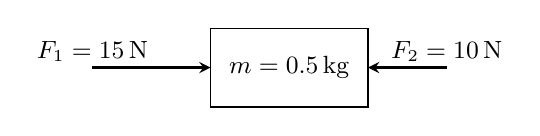
\begin{tikzpicture}
    \draw (0, 0) rectangle (2, 1) node [pos=0.5] {\small{$m = \SI{0.5}{\kilo\gram}$}};
    \draw [-stealth, thick] (-1.5, 0.5) -- (0, 0.5);
    \node at (-1.5, 0.7) {\small{$F_{1} = \SI{15}{\newton}$}};
    \draw [-stealth, thick] (3, 0.5) -- (2, 0.5);
    \node at (3, 0.7) {\small{$F_{2} = \SI{10}{\newton}$}};
\end{tikzpicture}
\end{document}